\DiaryEntry{Complex Analysis, 4 (Complex Integration)}{2026-04-23}{Complex Analysis}

\subsection{Curves}

We can define a curve in the complex $z$-plane as a complex function parametrized by a real parameter $t$,

\bee
z = z(t) = x(t) + jy(t), \quad t = [a,b]
\eee

The point $z(a)$ is the start point, the point $z(b)$ is the end point or terminal point of the curve, respectively.

A curve is said to be \emph{simple}, if it does not cross itself; ie $z(t_1) \neq z(t_2)$ for all different $t_1, t_2 \in [a,b]$. A curvie is \emph{closed}, if $z(a) = z(b)$. Combining these two characteristics, a curve is called a \emph{simple closed curve} or \emph{Jordan} curve, if it is closed and does not intersect (apart at the endpoints $z(a) = z(b)$).

\paragraph{Example: Line.} A line connecting two complex points $z_1, z_2$ is given by

\bee
z(t) = (1-t) z_1 + t z_2, \quad t \in [0,1]
\eee

\paragraph{Example: (Unit) Circle.} A circle with radius $r$ and center at the origin is given by

\bee
z(t) = r \cos(t) + j \sin(t), \quad t \in [0,2 \pi]
\eee

A closed curve (or contour) $\gamma$ is called \emph{positively oriented} (anticlockwise) if the interior domain lies to the left of an observer  tracing out the points in order; otherwise it is \emph{negatively oriented} (clockwise).

The Figure below shows a positively oriented curve; running anticlockwise along the curve (as indicated by the arrow), the interior lies on the left side.

\begin{figure}[H]
\centering
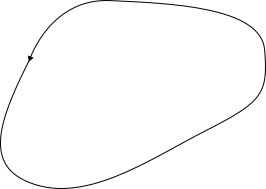
\includegraphics[scale=0.75]{images/2026-04-23-curve_01.png}
\end{figure}

\subsection{Complex Integration}

Complex integration of a function $f(z)$ is always along a curve $\gamma$; we calculate the values of $f(z)$ along the curve and integrate over them,

\bee
I = \int_\gamma f(z) dz
\eee

As described above, the curve $\gamma$ can be given as complex function $z(t)$ parametrized by a real parameter $t$,

\bee
z = z(t) = x(t) + jy(t), \quad t = [a,b]
\eee

In this case, the integral can be further developed into

\bee
I = \int_\gamma f(z) dz = \int_{a}^b f(z(t)) \frac{dz}{dt} dt
\eee



\paragraph{Example with analytic function.} We start with a simple example of the complex analytic function $w = f(z) = z^2$. We want to integrate from $z = 0$ to $z= 1+j$. We integrate along different curves (as we will show later, the curves do not matter as the function is analytic).

The first curve is along a straight line from $0 \rightarrow 1$, this yields the integral $I_{1,1}$, then along a straight line from $1 \rightarrow 1+j$ which yields the integral $I_{1,2}$.

For integration along $0 \rightarrow 1$, we have $z = t, t=0,\ldots 1$ and $dz = dt$. The integral $I_{1,1}$ therefore becomes

\begin{equation*}
    I_{1,1} = \int_0^1 (t)^2 dt = \cdots = \frac{1}{3}
\end{equation*}

For integration along $1 \rightarrow 1+j$, we have $z=1+jt, t=0,\ldots 1$ and $dz = j dt$. The integral $I_{1,2}$ therefore becomes

\begin{equation*}
    I_{1,2} = \int_0^1 (1 + jt)^2 j dt = \cdots = -1 + j\frac{2}{3}
\end{equation*}

Summing the two contributions finally yields

\begin{equation*}
    I_{1} = -\frac{2}{3} + j\frac{2}{3}
\end{equation*}

The second curve is a straight line between $0$ and $1+j$. We have $z = t + j t$ and therefore $dz = (1+j) dt$. Inserting into the integral yields

\begin{equation*}
    I_{2} = \int_0^1 (t + jt)^2 (1+j) dt = \cdots = -\frac{2}{3} + j\frac{2}{3}
\end{equation*}

As a last curve, we choose the parable $z = t + jt^2$. We have $\frac{dz}{dt} = 1 + 2jt \rightarrow dz = (1+2jt) dt$ and we obtain for the integral

\begin{equation*}
    I_{3} = \int_0^1 (t + jt^2)^2 (1+2jt) dt = \cdots = -\frac{2}{3} + j\frac{2}{3}
\end{equation*}

In all three cases, the integral gave the same value. This is due to the fact that the integrand is an analytic function.

\begin{verbatim}
(%i22)	p3:integrate((1+%i)*(t + %i*t)^2, t, 0, 1);
(p3)	(2*%i*(%i+1))/3
(%i23)	rectform(p3);
(%o23)	(2*%i)/3-2/3
(%i24)	p4:integrate((1+2*%i*t)*(t + %i*t^2)^2, t, 0, 1);
(p4)	(2*%i-2)/3
(%i25)	rectform(p4);
(%o25)	(2*%i)/3-2/3
\end{verbatim}

As a last step, we show that $f(z) = z^2$ is an analytic function. We have

\bee
f(z) = z^2 = (x + jy)^2 = x^2 - y^2 + 2jxy
\eee

so $u(x,y) = x^2 - y^2$ and $v(x,y) = 2xy$. The partial derivatives are

\bee
\frac{\partial u}{\partial x} = 2x, \quad \frac{\partial u}{\partial y} = -2y, \quad \frac{\partial v}{\partial x} = 2y, \quad \frac{\partial v}{\partial y} = 2x
\eee

Comparing with the Cauchy-Riemann equations \eqref{2026-01-13:eq1}, we see that

\bee
\frac{\partial u}{\partial x} = 2x = \frac{\partial v}{\partial y}, \quad \frac{\partial u}{\partial y} = -2y = - \frac{\partial v}{\partial x}
\eee

Both Cauchy-Riemann equations are satisfied for all $x, y \in \mathbb{R}$. Furthermore, the partial derivatives are continuous everywhere. Therefore, $f(z) = z^2$ is analytic in the entire complex plane. \qed


\paragraph{Example with non-analytic function.} We consider the function $w = u+jv = Re(z) = Re(x+jy) = x$. So $u(x,y) = x, v(x,y) = 0$. We will use the Cauchy-Rieman equations \eqref{2026-01-13:eq1}to show that the function is not analytic. We first calculate the partial derivatives,

\bee
    \frac{\partial u}{\partial x} = 1, \quad \frac{\partial u}{\partial y} = 0, \quad \frac{\partial v}{\partial x} = 0, \quad \frac{\partial v}{\partial y} = 0
\eee

Checking the Cauchy-Rieman equations, we see that the first condition does not hold and therefore the function is \emph{not} analytic,

\bee
\frac{\partial u}{\partial x} \neq \frac{\partial v}{\partial y}, \quad \frac{\partial u}{\partial y} = - \frac{\partial v}{\partial x}
\eee 


As in the previous example, we want to integrate from $z = 0$ to $z= 1+j$; this time the integral will be different as the function is not analytic.

The first curve is along a straight line from $0 \rightarrow 1$, this yields the integral $I_{1,1}$, then along a straight line from $1 \rightarrow 1+j$ which yields the integral $I_{1,2}$.

For integration along $0 \rightarrow 1$, we have $z = t, t=0,\ldots 1$ and $dz = dt$. The integral $I_{1,1}$ therefore becomes

\begin{equation*}
    I_{1,1} = \int_0^1 t dt = \cdots = \frac{1}{2}
\end{equation*}

For integration along $1 \rightarrow 1+j$, we have $z=1+jt, t=0,\ldots 1$ and $dz = j dt$. The integral $I_{1,2}$ therefore becomes

\begin{equation*}
    I_{1,2} = \int_0^1 1 \cdot j dt = \cdots = j
\end{equation*}

Summing the two contributions finally yields

\begin{equation*}
    I_{1} = \frac{1}{2} + j
\end{equation*}


The second curve is a straight line between $0$ and $1+j$. We have $z = t + j t$ and therefore $dz = (1+j) dt$. Inserting into the integral yields

\begin{equation*}
    I_{2} = \int_0^1 t (1+j) dt = \cdots = \frac{1}{2} + j \frac{1}{2}
\end{equation*}

As a last curve, we choose the parable $z = t + jt^2$. We have $\frac{dz}{dt} = 1 + 2jt \rightarrow dz = (1+2jt) dt$ and we obtain for the integral

\begin{equation*}
    I_{3} = \int_0^1 t (1+2jt) dt = \cdots = \frac{1}{2} + j\frac{2}{3}
\end{equation*}

In all three cases, the integral gave a different value which is due to the fact that the integrand is not an analytic function.


\subsection{Path Independence}

We have the following theorem.

\begin{theorem}
    Suppos that the function $f$ is continuous and has an antiderivative $F$ in the domain $\Sc$. If $a, b \in \Sc$ and $\gamma$ is a curve in $\Sc$ joining $a$ and $b$, then

    \bee
    \int_\gamma f(z) dz = F(b) - F(a)
    \eee

    The integral depends only on the points $a$ and $b$ and \emph{not} on the choice of $\gamma$. In particular, if $\gamma$ is closed in $\Sc$, then

    \bee
    \int_\gamma f(z) dz = 0
    \eee

\end{theorem}


%%% Local Variables:
%%% mode: latex
%%% TeX-master: "journal"
%%% End:
